\documentclass[12pt, a4paper]{article}
\usepackage{esvect}
\usepackage{amsmath}
\usepackage{eso-pic}
\usepackage{pdfpages}
\usepackage{graphicx}
\usepackage[utf8]{inputenc}
\usepackage[svgnames]{xcolor}
\usepackage{tcolorbox}
\usepackage{listings}
\usepackage{hyperref}
\usepackage{titling}
\usepackage{listings}
\lstset{breaklines=true,}
\usepackage[T1]{fontenc}
\newtheorem{def}{Definição}
\newtheorem{reso}{Resolução}
%\renewcommand*\familydefault{\sfdefault}

\title{Similaridade do Cosseno}

\author{Ronaldo Pacheco Pereira}

\begin{document}
\maketitle

\section{Similaridade do Cosseno}

A similaridade do cosseno é uma métrica de similaridade comumente empregada em diversas áreas, tais como aprendizado de máquina, processamento de linguagem natural e recuperação de informações. Essa métrica é fundamentada no ângulo entre dois vetores em um espaço n-dimensional e é calculada por meio da função de similaridade do cosseno.

\subsection{Cálculo da Similaridade do Cosseno}

A similaridade do cosseno é calculada usando a fórmula:

\[similarity(A, B) = \frac{A \cdot B}{\left\Vert A \right\Vert \cdot \left\Vert B \right\Vert}\]

\subsection{Interpretação da Similaridade do Cosseno}
A similaridade do cosseno é uma medida que varia de -1 a 1. Um valor de 1 indica que os dois vetores são idênticos (ângulo de 0º), enquanto um valor de -1 indica que os dois vetores são opostos (ângulo de 180º). Quando o valor é 0, isso significa que os vetores são ortogonais (ângulo de 90º).




\subsection{Aplicações em Data Science}

A similaridade do cosseno é amplamente utilizada em Data Science em diversas aplicações, tais como:


\begin{itemize}
    \item Recomendação de itens: é comum utilizar a similaridade do cosseno para calcular a similaridade entre os itens que os usuários visualizaram, compraram ou classificaram, a fim de sugerir outros itens semelhantes com base na similaridade de seus vetores de características;
    \item Agrupamento de texto: é possível utilizar a similaridade do cosseno para agrupar documentos de texto em conjuntos com base em suas similaridades, considerando cada documento como um vetor de termos. Isso é útil para análise de tópicos e detecção de spam;
    \item Detecção de plágio: a similaridade do cosseno é uma ferramenta eficaz para detecção de plágio em documentos de texto, comparando a similaridade entre o documento original e o documento suspeito;
    \item Análise de sentimentos: a similaridade do cosseno pode ser usada para medir a semelhança entre palavras ou expressões em um corpus de textos, auxiliando na análise de sentimentos ou na identificação de sinônimos e antônimos;
    \item Classificação de imagens: a similaridade do cosseno pode ser usada para comparar vetores de características extraídos de imagens, a fim de classificá-las em categorias semelhantes com base em sua similaridade.
    
\end{itemize}
Esses são apenas alguns exemplos de como a similaridade do cosseno pode ser aplicada em Data Science. Ela é uma métrica útil para lidar com problemas em que a similaridade entre dois itens é importante, especialmente em casos em que os dados são esparsos e de alta dimensionalidade.
\section{PyCharm IDE Python}

Para esse trabalho, utilizei a IDE PyCharm (Python).
O PyCharm é um IDE para Python, disponível em duas edições, Community e Professional. Ele possui recursos para autocompletar código, depuração, refatoração, testes automatizados e integração com controle de versão. O PyCharm inclui um gerenciador de projetos, terminal integrado e suporte a diferentes interpretes Python e ambientes virtuais. Além disso, oferece suporte a plugins para desenvolvimento em outras linguagens e plataformas. O PyCharm é amplamente utilizado por programadores e equipes de desenvolvimento em todo o mundo.


\section{Bibliotecas utilizadas em Python}
Abaixo a relação de bibliotecas utilizadas nesse trabalho.
\begin{center}
    \includegraphics[width=14cm]{fig1_1.png}
\end{center}

\textbf{TfidfVectorizer:}\\
Essa ferramenta é usada para obter informações relevantes de texto de um conjunto de documentos. Ela avalia o valor TF-IDF (frequência de termo–inverso da frequência nos documentos) para cada termo em cada documento, o que é uma medida estatística da importância de uma palavra em um documento.\\

\textbf{cosine\_similarity:}\\
\text{}Utilizada para calcular a similaridade do cosseno entre dois vetores. Isso possibilita comparar a similaridade entre diferentes documentos.\\

\textbf{MatPlotLib.Pyplot:}\\
Matplotlib.pyplot é um módulo do pacote Matplotlib para criação de gráficos em Python. Ele fornece funções simples e intuitivas para criação de diversos tipos de visualizações, como gráficos de linhas, de dispersão e de barras, permitindo a adição de títulos e legendas aos gráficos, ajuste de escala dos eixos, criação de múltiplos gráficos em uma única figura e salvamento dos gráficos em diversos formatos. O pyplot é frequentemente utilizado em conjunto com outras bibliotecas de análise de dados em Python, como NumPy e Pandas, tornando-se uma ferramenta essencial para análise e interpretação de dados.\\

\textbf{pandas:}\\
Pandas é uma biblioteca de análise de dados em Python, que fornece estruturas de dados flexíveis e eficientes para manipulação e análise de dados tabulares. Com pandas, é possível realizar diversas operações em dados, como limpeza, transformação, seleção e agregação, tornando-se uma ferramenta essencial para análise de dados em Python..

\subsection{Dados Qualitativos}
Os Dados foram baixados no site Kaggle e após ser limpo de inconsistências e erros, foi importado e agregado usando o pandas no formato final Xlsx, deixando assim, somente a informação util ao trabalho final.


\subsection{Texto em Vetor}
A partir dos dados limpos, transformaremos cada frase em um vetor numérico. 

\begin{tcolorbox}[colback=blue!20, colframe=gray!20]
\begin{lstlisting}[language=Python]
vetorizador = TfidfVectorizer()

# vetorizar as descricoes dos produtos
vetores = vetorizador.fit_transform(dados_texto))
\end{lstlisting}
\end{tcolorbox}

\begin{center}
    \includegraphics[width=14cm]{fig2.png}
\end{center}

\subsection{Transformar o input do usuário em Vetor numérico}
Nesse trabalho, sugeri ao usuário que informe a marca, modelo ou material do relógio a ser verificado. 
\begin{tcolorbox}[colback=blue!20, colframe=gray!20]
\begin{lstlisting}[language=Python]
# exemplo de relógio fornecido pelo usuário
relogio_usuario = input('Digite a marca, modelo ou material do relogio que você quer verificar a similaridade (separados por espaço): ').split()

# transformar o exemplo em um vetor numérico
relogio_usuario_vetor = vetorizador.transform([' '.join(map(str, relogio_usuario + [''] * (len(dados_selecionados.columns) - len(relogio_usuario))))])
\end{lstlisting}
\end{tcolorbox}


\subsection{Similaridade}
A similaridade do cosseno é obtido pelo código baixo citado.
A função recebe a variável e retorna uma matriz de similaridade entre o que foi pesquisado e o que consta no arquivo.

\begin{tcolorbox}[colback=blue!20, colframe=gray!20]
\begin{lstlisting}[language=Python]
similaridades = cosine_similarity(relogio_usuario_vetor, vetores)
indices_similares = similaridades.argsort()[0][::-1]
# selecionar os 10 relógios mais similares, excluindo aqueles com a mesma marca que o exemplo dado
marca_usuario = relogio_usuario[0]
top_similares = []
for i in indices_similares:
    if dados.loc[i, 'Brand'] != marca_usuario:
        top_similares.append(i)
    if len(top_similares) >= 10:
        break

# imprimir os 10 relógios mais similares
print("Os 10 relógios mais similares a", ' '.join(map(str, relogio_usuario)), "são:")

for i in top_similares:
    print(dados.loc[i, ['Brand', 'Model', 'Case_mat_strap', 'Type', 'price']])
# adicionar as colunas de similaridade do cosseno e ângulo do cosseno
dados_selecionados.loc[:, 'Cosine Similarity'] = similaridades[0]
dados_selecionados.loc[:, 'Cosine Angle'] = [math.degrees(math.acos(similarity)) for similarity in similaridades[0]]

# imprimir os 10 Relogios mais similares com as colunas adicionais
print(dados_selecionados.loc[top_similares, ['Brand', 'Model', 'price', 'Cosine Similarity', 'Cosine Angle']])
\end{lstlisting}
\end{tcolorbox}



Abaixo uma visualização de parte do resultado quando a pesquisa feita foi pelo material Titanium.

\begin{center}
    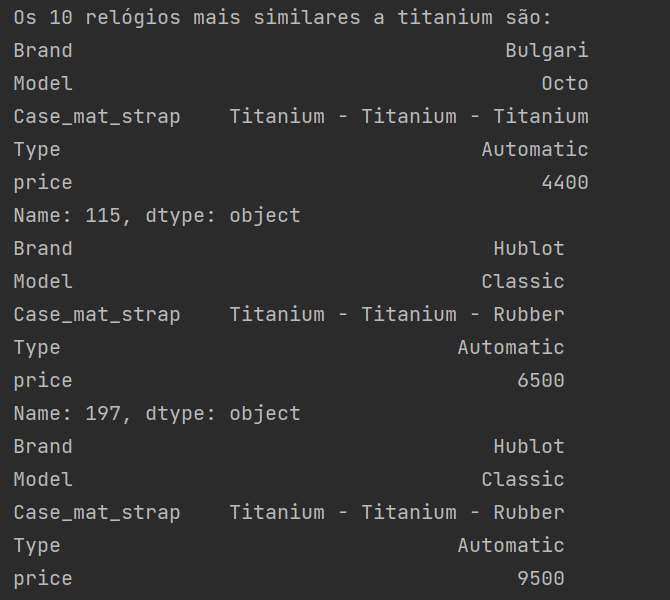
\includegraphics[width=14cm]{fig3.png}
\end{center}

\subsection{Finalização}
Por fim, para visualizar a similaridade de cosseno e o angulo do cesseno temos o código abaixo.

\begin{tcolorbox}[colback=blue!20, colframe=gray!20]
\begin{lstlisting}[language=Python]
vetores_similares = vetores[top_similares]

# calcular os ângulos dos vetores
angulos = []
for vetor in vetores_similares:
    angulo = np.arccos(cosine_similarity(relogio_usuario_vetor, vetor)[0][0]) * 180 / np.pi
    angulos.append(angulo)
# extrair as coordenadas dos vetores dos 10 relógios mais similares
coordenadas_similares = vetores_similares.toarray()
# adicionar as colunas de similaridade do cosseno e ângulo do cosseno
dados_selecionados['Cosine Similarity'] = similaridades[0]
dados_selecionados['Cosine Angle'] = [math.degrees(math.acos(similarity)) for similarity in similaridades[0]]
print("Os relogios mais similares a ", ' '.join(map(str, relogio_usuario)), "são:")
display(dados_selecionados.loc[top_similares, ['Brand', 'Model', 'Cosine Similarity', 'Cosine Angle']])
# extrair as coordenadas dos vetores dos 10 relógios mais similares
coordenadas_similares = vetores_similares.toarray()

plt.show()
\end{lstlisting}
\end{tcolorbox}
\begin{center}
    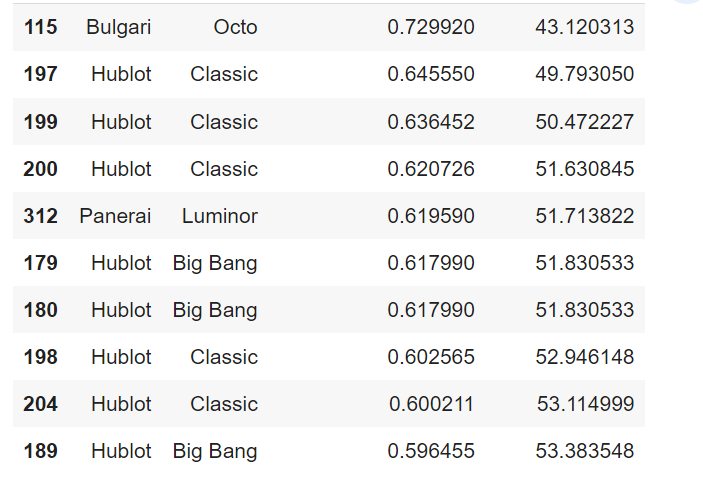
\includegraphics[width=14cm]{fig4.png}
\end{center}
\begin{center}
    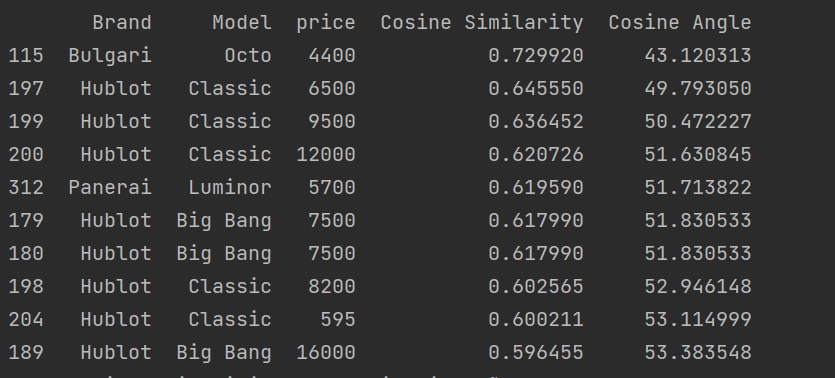
\includegraphics[width=14cm]{fig5.png}
\end{center}

\end{document}
